%%
\documentclass[sigconf,review]{acmart}
\usepackage[utf8]{inputenc}
\usepackage{listings}

\graphicspath{{figs/}{}}

%%
%% \BibTeX command to typeset BibTeX logo in the docs
\AtBeginDocument{%
  \providecommand\BibTeX{{%
    Bib\TeX}}}

%% Rights management information.  This information is sent to you
%% when you complete the rights form.  These commands have SAMPLE
%% values in them; it is your responsibility as an author to replace
%% the commands and values with those provided to you when you
%% complete the rights form.
\setcopyright{acmcopyright}
\copyrightyear{2023}
\acmYear{2023}
\acmDOI{XXXXXXX.XXXXXXX}

%% These commands are for a PROCEEDINGS abstract or paper.
\acmConference[TTC'23]{15th Transformation Tool Contest}{July 20, 2023}{Leicester, UK}
%%
%%  Uncomment \acmBooktitle if the title of the proceedings is different
%%  from ``Proceedings of ...''!
%%
%%\acmBooktitle{Woodstock '18: ACM Symposium on Neural Gaze Detection,
%%  June 03--05, 2018, Woodstock, NY}
\acmPrice{0.00}
\acmISBN{978-1-4503-XXXX-X/18/06}


%%
%% Submission ID.
%% Use this when submitting an article to a sponsored event. You'll
%% receive a unique submission ID from the organizers
%% of the event, and this ID should be used as the parameter to this command.
%%\acmSubmissionID{123-A56-BU3}

%%
%% For managing citations, it is recommended to use bibliography
%% files in BibTeX format.
%%
%% You can then either use BibTeX with the ACM-Reference-Format style,
%% or BibLaTeX with the acmnumeric or acmauthoryear sytles, that include
%% support for advanced citation of software artefact from the
%% biblatex-software package, also separately available on CTAN.
%%
%% Look at the sample-*-biblatex.tex files for templates showcasing
%% the biblatex styles.
%%

%%
%% The majority of ACM publications use numbered citations and
%% references.  The command \citestyle{authoryear} switches to the
%% "author year" style.
%%
%% If you are preparing content for an event
%% sponsored by ACM SIGGRAPH, you must use the "author year" style of
%% citations and references.
%% Uncommenting
%% the next command will enable that style.
%%\citestyle{acmauthoryear}

% From https://tex.stackexchange.com/questions/152829/

\newcommand\YAMLcolonstyle{\color{red}\mdseries}
\newcommand\YAMLkeystyle{\color{black}\bfseries}
\newcommand\YAMLvaluestyle{\color{blue}\mdseries}

\makeatletter

% here is a macro expanding to the name of the language
% (handy if you decide to change it further down the road)
\newcommand\language@yaml{yaml}

\expandafter\expandafter\expandafter\lstdefinelanguage
\expandafter{\language@yaml}
{
  keywords={true,false,null,y,n},
  keywordstyle=\color{darkgray}\bfseries,
  basicstyle=\YAMLkeystyle,                                 % assuming a key comes first
  sensitive=false,
  comment=[l]{\#},
  morecomment=[s]{/*}{*/},
  commentstyle=\color{purple}\ttfamily,
  stringstyle=\YAMLvaluestyle\ttfamily,
  moredelim=[l][\color{orange}]{\&},
  moredelim=[l][\color{magenta}]{*},
  moredelim=**[il][\YAMLcolonstyle{:}\YAMLvaluestyle]{:},   % switch to value style at :
  morestring=[b]',
  morestring=[b]",
  literate =    {---}{{\ProcessThreeDashes}}3
                {>}{{\textcolor{red}\textgreater}}1     
                {|}{{\textcolor{red}\textbar}}1 
                {\ -\ }{{\mdseries\ -\ }}3,
}

% switch to key style at EOL
\lst@AddToHook{EveryLine}{\ifx\lst@language\language@yaml\YAMLkeystyle\fi}
\makeatother

\newcommand\ProcessThreeDashes{\llap{\color{cyan}\mdseries-{-}-}}


%%
%% end of the preamble, start of the body of the document source.
\begin{document}

%%
%% The "title" command has an optional parameter,
%% allowing the author to define a "short title" to be used in page headers.
\title{Asymmetric and Directed Bidirectional Transformation for Container Orchestrations}

%%
%% The "author" command and its associated commands are used to define
%% the authors and their affiliations.
%% Of note is the shared affiliation of the first two authors, and the
%% "authornote" and "authornotemark" commands
%% used to denote shared contribution to the research.
\author{Antonio Garcia-Dominguez}
%\authornote{Both authors contributed equally to this research.}
\email{a.garcia-dominguez@york.ac.uk}
\orcid{0000-0002-4744-9150}
\affiliation{%
  \institution{University of York}
  \streetaddress{Deramore Lane, Heslingon}
  \city{York}
  \country{UK}
  \postcode{YO10 5GH}
}

%%
%% By default, the full list of authors will be used in the page
%% headers. Often, this list is too long, and will overlap
%% other information printed in the page headers. This command allows
%% the author to define a more concise list
%% of authors' names for this purpose.
\renewcommand{\shortauthors}{Garcia-Dominguez}

%%
%% The abstract is a short summary of the work to be presented in the
%% article.
\begin{abstract}
  In many DevOps scenarios, tools operate from declarative models of intended
  system configuration (e.g. Ansible/Puppet/Chef descriptions of
  infrastructure-as-code, or Kubernetes and Docker Compose descriptions of
  orchestrations of containers). DevOps-oriented domain-specific modeling
  notations will typically only cover a subset of all the capabilities in these
  configuration formats: this means users will need to manually edit the
  configuration files generated from the higher-level models. In many editing
  sessions, users will also touch upon parts that came from the high-level
  model, and will want that high-level model to be updated accordingly.
  Likewise, a user may want to introduce a change through the high-level model
  and not lose the YAML customisations that are unrelated to the high-level
  model. These requirements imply a need for a bidirectional transformation
  (``bx'') which is asymmetric (the configuration file contains all the
  information in the high-level model and more), and directed (changes are only
  applied to one side at a time). This case proposes revisiting the current
  state of bx tools for asymmetric and directed transformations, and complements
  the prior Families to Persons case from TTC 2017, which focused on a
  symmetrical and directed transformation. The case will reuse the Benchmarx
  framework from the TTC 2017 case.
\end{abstract}

\begin{CCSXML}
  <ccs2012>
  <concept>
  <concept_id>10011007.10011006.10011050.10011017</concept_id>
  <concept_desc>Software and its engineering~Domain specific languages</concept_desc>
  <concept_significance>500</concept_significance>
  </concept>
  </ccs2012>
\end{CCSXML}

\ccsdesc[500]{Software and its engineering~Domain specific languages}

%%
%% Keywords. The author(s) should pick words that accurately describe
%% the work being presented. Separate the keywords with commas.
\keywords{container orchestration, bidirectional transformations, model merging, graphical models, YAML}
%% A "teaser" image appears between the author and affiliation
%% information and the body of the document, and typically spans the
%% page.
%% \begin{teaserfigure}
%%   \includegraphics[width=\textwidth]{sampleteaser}
%%   \caption{Seattle Mariners at Spring Training, 2010.}
%%   \Description{Enjoying the baseball game from the third-base
%%   seats. Ichiro Suzuki preparing to bat.}
%%   \label{fig:teaser}
%% \end{teaserfigure}

%% \received{20 February 2007}
%% \received[revised]{12 March 2009}
%% \received[accepted]{5 June 2009}

%%
%% This command processes the author and affiliation and title
%% information and builds the first part of the formatted document.
\maketitle

\section{Introduction}

DevOps was defined by Leite et al.~\cite{leite_survey_2020} as a ``collaborative
and multidisciplinary effort within an organization to automate continuous
delivery of new software versions, while guaranteeing their correctness and
reliability''. The rising interest in DevOps (with over 10\% of the 61,302
responses to the Stack Overflow 2022 Developer
Survey\footnote{\url{https://survey.stackoverflow.co/2022/}} considering
themselves ``DevOps specialists'') has motivated the creation of a number of
domain-specific modelling notations for it, covering aspects such as
microservice architectures~\cite{sorgalla_applying_2021}, DevOps
processes~\cite{colantoni_devopsml_2020}, or multi-cloud
applications~\cite{ferry_cloudmf_2018}.

At a technical level, the automated continuous delivery efforts in DevOps
typically require using tools to automate deployment. These include
infrastructure-as-code tools (e.g.
Puppet\footnote{\url{https://www.puppet.com/}} or
Ansible\footnote{\url{https://www.ansible.com/}}), and container orchestration
tools such as Kubernetes\footnote{\url{https://kubernetes.io/}} or Docker
Compose\footnote{\url{https://docs.docker.com/compose/}}. Many of these tools
operate by reading a declarative description of the desired system state or the
intended combination of containers, usually written in a structured format
(e.g.\ YAML\footnote{\url{https://yaml.org/}}) according to a loosely defined
schema (c.f.\ the Docker Compose file format reference, which evolves from
version to
version\footnote{\url{https://docs.docker.com/compose/compose-file/}}).

It stands to reason that DevOps model-driven approaches would often aim to
generate at least some of these configuration files from the high-level
descriptions of the intended service compositions. Most likely, the high-level
descriptions will only model the subset of the capabilities of the underlying
tools that is relevant for their abstractions, as trying to capture all
capabilities would overcomplicate the models and make them more brittle to minor
changes in the underlying configuration file formats. From this limitation, it
follows that users would typically manually customise the generated
configuration files to cover the aspects not described by the high-level model.
Users may later want to update the high-level model from the configuration file,
to use it for visualisation (e.g.\ for onboarding new developers) or for
reorganising the system in a more approachable notation with domain-specific
validation rules.

This paper proposes a case based on the above scenario, focusing on container
orchestration with Docker Compose. A high-level graphical domain-specific model
(implemented with Sirius) is transformed into a Docker Compose YAML file, which
can be customised by the user using a plain text editor. The high-level model
can be updated from the YAML file at any time. It should also be possible to
edit the high-level model and push the changes to the YAML file, while retaining
any elements that were not part of the high-level graphical DSML.

At an essential level, this case implies the definition of a bidirectional
transformation (``bx'' from now on) between the high-level DSML and Docker
Compose YAML files. In TTC 2017, the Families to Persons case by Anjorin et
al.~\cite{anjorin_families_2017} evaluated the available approaches for
symmetric and directed bx using the proposed Benchmarx framework. This work was
later updated and expanded upon in a journal
paper~\cite{anjorin_benchmarking_2020}, which also collected a number of useful
terms to describe bx, as well as a feature model to cover the variability of bx
tools. Families to Persons was symmetric (neither side was a view of the other,
with information loss happening in both directions), and directed
(consistency-relevant changes were only applied to one side at a time). The
proposed case is still directed, but it is asymmetrical (the Docker Compose YAML
file contains strictly more information than the high-level model, so
information loss only happens in one direction). While this should make it
conceptually ``easier'' than the symmetric Families to Persons bx, the mapping
is also more complicated, with some objects in the high-level model being turned
into simple string concatenations in the target model. At the same time, it can
be argued that the generation of Docker Compose YAML files is a more
industrially relevant scenario: if the current state of the art in bx tools
(which may have significantly evolved since the TTC 2017 case) can handle it
well, this could prove to be an interesting application niche.

\section{Modeling Languages}

\begin{figure}
  \centering
  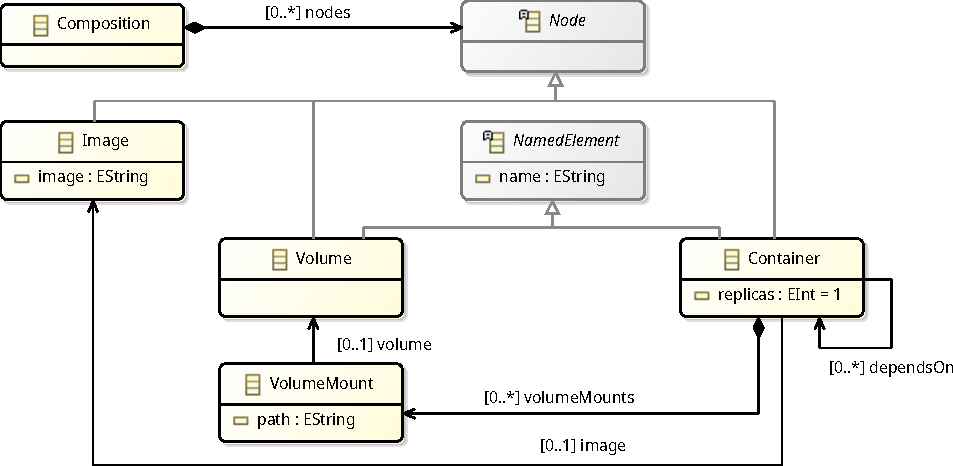
\includegraphics[width=\columnwidth]{containers-metamodel}
  \caption{Class diagram for the Containers metamodel}%
  \label{fig:containers-metamodel}
\end{figure}

\begin{figure}
  \centering
  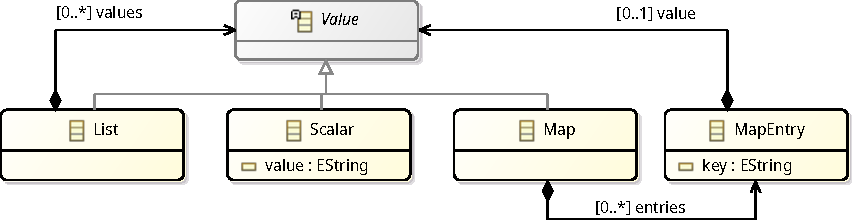
\includegraphics[width=\columnwidth]{miniyaml-metamodel}
  \caption{Class diagram for the MiniYAML metamodel}%
  \label{fig:miniyaml-metamodel}
\end{figure}

The proposed bx is between two languages: a ``Containers'' domain-specific
modelling language (shown in Figure~\ref{fig:containers-metamodel}), and a
simplification of the YAML data model called ``MiniYAML'' (shown in
Figure~\ref{fig:miniyaml-metamodel}).

\subsection{Abstract syntax}
\label{sec:abstract-syntax}

\newcommand*{\metaclass}[1]{\textsc{#1}}
\newcommand*{\feature}[1]{\texttt{#1}}

Models conforming to the Containers metamodel
(Figure~\ref{fig:containers-metamodel}) have a \metaclass{Composition} as their
root object, containing a number of \metaclass{Node}s of various types. An
\metaclass{Image} represents a specific Docker image by its full name including
the registry (if it is not the Docker Hub) and tag, as stored in its
\feature{image} attribute. A \metaclass{Container} is a component that runs one
or more \feature{replicas} of a certain \metaclass{Image}. A
\metaclass{Container} may have \metaclass{Volume\-Mount}s of certain
\metaclass{Volume}s (units of persistent storage) at specific \feature{path}s.
\metaclass{Container}s and \metaclass{Volume}s are \metaclass{NamedElement}s,
which have a \feature{name} that also acts as their unique identifier. A
\metaclass{Container} may \feature{dependOn} other \metaclass{Container}s,
meaning that it should only be started after its dependencies have been started.

On the other hand, a model conforming to the MiniYAML metamodel
(Figure~\ref{fig:miniyaml-metamodel}) has a \metaclass{Map} as its root object,
which contains \metaclass{MapEntry} objects. Each \metaclass{MapEntry} has a
\feature{key} (a string, which should be unique within its containing
\metaclass{Map}), and a \feature{value}. Besides \metaclass{Map}, other types of
\metaclass{Value}s include \metaclass{List}s (of \metaclass{Value}s), and
\metaclass{Scalar} values with a string (this is a simplification from YAML,
which can support integer and floating point types through its JSON schema).

\subsection{Concrete syntax}
\label{sec:concrete-syntax}

\newcommand*{\eclipseproject}[1]{\texttt{#1}}
\newcommand*{\javaclass}[1]{\textsc{#1}}

\begin{figure*}
  \centering
  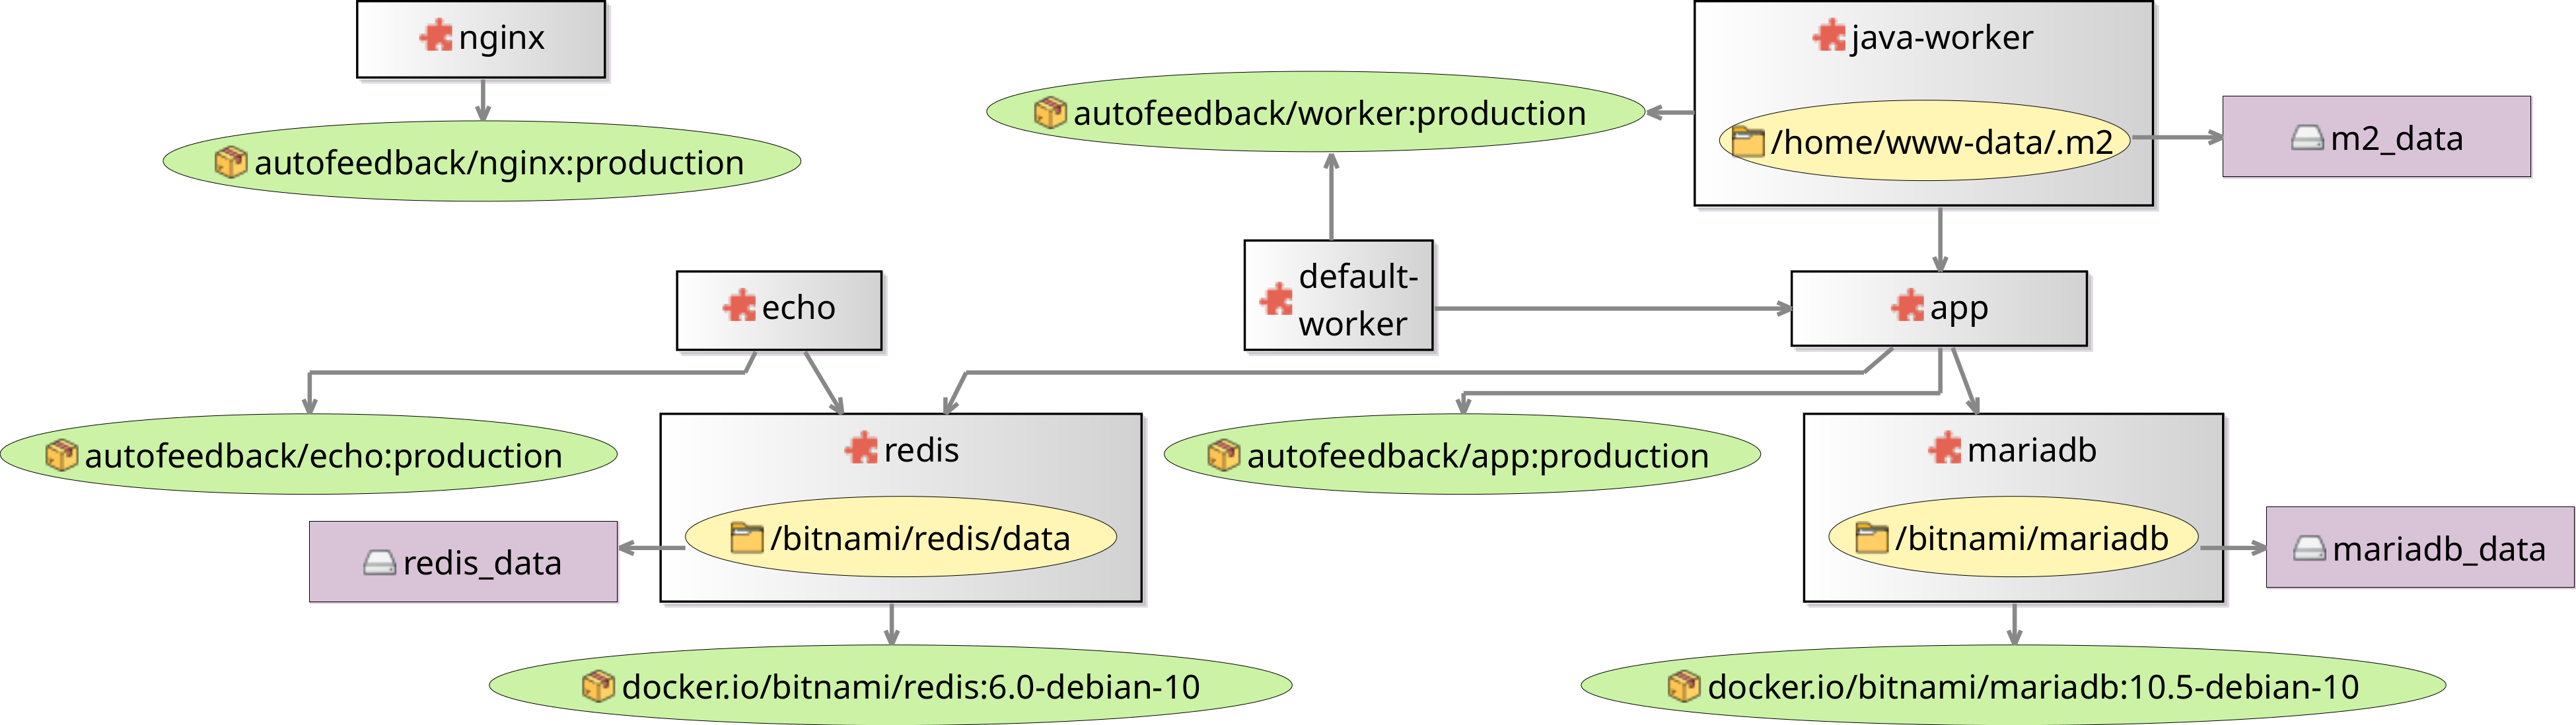
\includegraphics[width=\textwidth]{containers-model}
  \caption{Example containers model, based on the AutoFeedback open-source system}%
  \label{fig:containers-model}
\end{figure*}

The concrete syntax of the Containers modelling language is implemented through
Eclipse Sirius\footnote{\url{https://www.eclipse.org/sirius/}} and exemplified
in Figure~\ref{fig:containers-model}, which models the container orchestration
used by the AutoFeedback system developed by the
author\footnote{\url{https://gitlab.com/autofeedback/autofeedback-webapp/-/blob/master/docker-compose.yml}}.
\metaclass{Container}s are grey rectangles decorated with a puzzle piece icon,
labelled after their \feature{name}. A \metaclass{Container} may contain yellow
ovals representing their \metaclass{Volume\-Mount}s, labelled after their
\feature{path}s and decorated with a folder icon. An \metaclass{Image} is
reflected as a green oval with a cardboard box icon, labelled after their
\feature{image}. \metaclass{Volume}s are purple rectangles with a hard disk
icon, labelled after their \feature{name}. Note that the \feature{replicas} of a
\metaclass{Container} is not part of its graphical syntax, but can be edited
through the Properties view of the Sirius editor.

\lstinputlisting[language=yaml,columns=flexible,float,caption={Example YAML from Figure~\ref{fig:containers-model}},label=lst:yaml-example]{listings/MyContainers.yml}

The MiniYAML language does not have an explicitly defined concrete syntax: while
the case artifact includes a tree-based editor autogenerated from the metamodel,
the ultimate concrete syntax is YAML itself. The case artifact includes an
\eclipseproject{uk.ac.york.ttc.mini\-yaml.model\-2yaml} project with a
\javaclass{MiniYAMLConverter} Java class which uses
SnakeYAML\footnote{\url{https://bitbucket.org/snakeyaml/snakeyaml}} to
automatically convert between Mini\-YAML models in XMI format, and YAML files.

\section{Intended Transformations}

The general intent of the transformation is to start from a model as the one in
Figure~\ref{fig:containers-model}, and produce a YAML document such as the one
in Listing~\ref{lst:yaml-example}. This YAML document can be edited manually in
various ways: a user could do a find-and-replace to rename a given container, or
they could add extra options for a given container or volume which are not part
of the Containers metamodel. It should be possible for the user to update the
Containers model from the YAML file at any point. It should also be possible to
edit a Containers model and update the YAML file from it, while keeping any
customisations that are unrelated to the Containers metamodel.

\subsection{High-level description}

In its forward direction (from Containers to MiniYAML), operating in batch mode
(where the MiniYAML model does not exist yet), the transformation should follow
these rules:

\begin{enumerate}
\item A \metaclass{Composition} should be transformed into a \metaclass{Map}
  with three keys: \feature{version} set to a ``2.4'' \metaclass{Scalar},
  \feature{services} set to a \metaclass{Map} whose \metaclass{MapEntry} objects
  are produced from the \metaclass{Container}s, and \feature{volumes} set to a
  \metaclass{Map} produced from the \metaclass{Volume}s.

\item A \metaclass{Container} should be transformed into a \metaclass{MapEntry}
  where the \feature{key} is equal to its \feature{name}. The value of the
  \metaclass{MapEntry} should be a \metaclass{Map} of its own, with at least the
  \feature{image} key set to the \feature{image} of the \metaclass{Image} of the
  \metaclass{Container}.

  The \metaclass{Map} may also have keys for:
  \begin{itemize}
  \item \feature{replicas}, if the value is different from 1.
  \item \feature{volumes}, set to a \metaclass{List} produced from the
    \metaclass{VolumeMount}s of the \metaclass{Container}.
  \item \feature{depends\_on}, set to a \metaclass{List} of \metaclass{Scalar}s
    with the names of the \metaclass{Container}s that this \metaclass{Container}
    depends upon.
  \end{itemize}

\item A \metaclass{VolumeMount} should be transformed into a \metaclass{Scalar}
  whose value should be of the form ``volumeName:path''.

\item A \metaclass{Volume} should be turned into a \metaclass{MapEntry} whose
  \feature{key} should be its \feature{name}. The \metaclass{MapEntry} should
  not have a value.
\end{enumerate}

If the MiniYAML model already exists before running the transformation forward,
then the containers, volumes, volume mounts, replicas, and inter-container
dependencies of the Containers model should replace those of the MiniYAML model,
while preserving any other elements outside the Containers metamodel (e.g.\ a
custom \feature{restart} entry in a container's \metaclass{Map}). At the very
least, adding or removing one of these elements from the Containers model should
add or remove the relevant element in the MiniYAML model. Ideally, the
transformation should be able to handle the renaming of a \metaclass{Container}
or \metaclass{Volume} while preserving the additional content that is unrelated
to the Containers metamodel. Furthermore, the transformation should minimise
unnecessary changes in the YAML file (e.g.\ changes in the order of the map
entries).

In its backward direction (from MiniYAML to Containers) in batch mode, the
transformation should recover the \metaclass{Composition}s, \metaclass{Image}s,
\metaclass{Volume}s and \metaclass{VolumeMount}s from the same MiniYAML elements
that would have been produced in the forward direction. These will replace the
contents of the Containers model entirely. Ideally, the transformation should
minimise unnecessary changes (e.g.\ changing the path of an \metaclass{Image} in
the model, which would cause unnecessary changes in the Sirius diagrams).

\subsection{Reference implementation}

\newcommand*{\file}[1]{\texttt{#1}}

Besides the above high-level description, the case materials include EMF-based
implementations of the Containers and MiniYAML metamodels, and a reference
implementation of the transformation using a combination of languages from the
Eclipse Epsilon open-source project:

\begin{itemize}
\item An ETL (Epsilon Transformation Language) script transforming Containers
  models to MiniYAML models (\file{con\-tai\-ners\-2\-miniyaml.etl}).

\item An ETL script transforming MiniYAML models to Containers models
  (\file{miniyaml2containers.etl}).

\item A combination of an Epsilon Merging Language (EML) script, an Epsilon
  Comparison Language (ECL) script, and an ETL script which can merge two
  MiniYAML models together (\file{mergeMiniyaml.eml},
  \file{compareMiniyaml.ecl}, and \file{mergeMiniyaml.etl}) respectively.

  In this transformation, the ``left'' MiniYAML model is the ``prioritary'' one:
  its containers, volumes, volume mounts, replicas, and inter-container
  dependencies will take precedence over those of the ``right'' MiniYAML model.
  Any other content (e.g.\ customisations outside the Containers metamodel) will
  be merged.

  At a high-level, the ECL script computes a match between the ``left'' and
  ``right'' models based on name-based paths
  (e.g.\ \feature{services.redis.image}), where \metaclass{Scalar}s also
  consider their value. The EML script merges matching elements together, and
  the ETL script copies non-matching elements from either side.
\end{itemize}

These transformations are then encapsulated as Java classes:

\begin{itemize}
\item \javaclass{ContainersToMiniYAML} implements the batch forward
  transformation, \javaclass{MergingContainersToMiniYAML} implements the forward
  transformation with merging if the MiniYAML model already exists, and
  \javaclass{MergingContainersToYAML} class implements the forward
  transformation with merging if the YAML file already exists.

\item \javaclass{MiniYAMLToContainers} implements the batch backward
  transformation from a MiniYAML model to a Containers model, and
  \javaclass{YAMLToContainers} also transforms the YAML file into a MiniYAML
  model before transforming it into a Containers model. The reference
  implementation does not have a ``merging'' version of the backward
  transformation: it replaces the Containers model if it exists.

\end{itemize}

\section{Research questions}

The aim of this case is to explore the capabilities of the current state of the
art of transformation tools in an asymmetric and directed bx. Specifically, the
case is intended to answer these questions:

\begin{enumerate}
\item How concisely can we specify such a bx with current tools?

  Having to maintain separate one-way transformations as in the reference
  implementation would incur significant cost when scaling up to the full
  complexity of real-world metamodels. Ideally, it should be possible to
  implement the bx through a single set of relationships, without repetition.
  This could be done through explicit consistency relationships, through triple
  graph grammars, or through static analysis of a one-way transformation (with
  perhaps some use of heuristics).

\item How well can such a bx preserve customisations in the YAML which are
  outside of the bx, across various types of changes in the models?

  The reference implementation can handle well the case where elements are added
  and removed, but it cannot handle renames well: renaming a container in the
  Containers model would most likely result in losing the additional content in
  the YAML file. A bx tool that can operate with operational deltas
  (``o-deltas'') would most likely be able to handle this case in a more robust
  manner.

\item How would such a bx scale to larger models, with more containers, more
  volumes, and more custom YAML elements outside of the transformation's
  control?

  In the reference implementation, the merging process of the MiniYAML model
  newly created from the Containers model with the previously existing (and
  potentially customised) MiniYAML model requires pairwise object matching, with
  $O(n^2)$ path comparisons per type. Is such a cost unavoidable, or are there
  more efficient ways to establish and maintain the relationships between the
  Containers and MiniYAML models?

\end{enumerate}

In practice, it is unlikely that the YAML documents will grow particularly
large\footnote{The average size of the \file{composer.yaml} files in the
\file{docker/awesome-compose} Github project is 609B:
\url{https://github.com/docker/awesome-compose.}}. Performance would likely not
be an issue for this bidirectional transformation. Instead, maintainability and
keeping to the principles of ``least change'' and ``least surprise'' would be
the most important aspects to tackle.

\section{Evaluation criteria}

Solutions will be evaluated across the following criteria:

\begin{enumerate}
\item \emph{Correctness}: following the approach from the authors of the
  Benchmarx benchmark~\cite{anjorin_benchmarking_2020}, test cases will check
  that the dependent model is consistent with the master model. This means that
  they should have the same containers, volumes, volume mounts, and images.

  This criteria will be measured according to the \% of test cases that are
  passed. The test cases will cover various scenarios, e.g.\ an initial
  ``batch'' execution in either direction, or the update of the dependent side
  after a certain change in the master side.

\item \emph{Conciseness}: a more concise description of the transformation
  should in principle be more maintainable. Since the statement structure can be
  significantly different across language, this criteria will be measured as the
  number of words in the transformation rules, ignoring comments. This is the
  same approach that was followed in the Families to Persons study cited above.

  For reference, the reference implementation includes a \file{count-words.sh}
  script which uses the C preprocessor to remove comments for Epsilon / Java
  programs. In its current version, the reference implementation uses 749 words
  in its Java code, 480 words in ETL, 162 words in EML, 81 words in EOL and 84
  words in ECL, for a total of 1556 words.

\item \emph{Least Change}: beyond just correctness, the transformations should
  avoid making any unnecessary changes that do not impact the consistency of the
  master and dependent model. For instance, in the forward direction, they
  should preserve the additional information in the existing YAML file, and the
  relative order of the keys in the YAML document. In the backward direction,
  they should also preserve the locations of the various nodes, avoiding
  disturbing existing Sirius diagrams whenever possible.

  This will be measured by checking in each test case the number of differences
  between the actual output and the expected output that do not impact
  consistency (e.g. YAML keys in a different relative position, or missing YAML
  keys that are unrelated to the transformation). Ideally, no such differences
  should be produced.

\end{enumerate}

% Restructure repo to be a fork of https://github.com/eMoflon/benchmarx

\section{Target prizes}

The prizes will be basted on a combination of the three criteria above. The
``Most Complete'' prize will go to the solution that passes the most tests
(resolving ties using the ``Least Change'' criterion). The ``Most Concise''
prize will go to the solution that requires the last words, while still passing
the correctness tests for adding and deleting elements (the tests for renaming
elements will not be considered).

If there are enough solutions, an overall ranking can be devised by adding their
rankings in each category, and sorting in ascending order. Ties will be resolved
by soring in ascending order of standard deviation (therefore, a tool that is
2nd/2nd would be ranked above a tool that is 1st/3rd). Further ties will be
resolved by the case author and TTC organizers.

\section{Journal-quality solution criteria}

To be eligible for a follow-up journal publication, a solution must be correct
in regard to addition and removal of containers, volumes, volume mounts, and
images. Conciseness and ``least change'' are desirable properties, but not
required for such a publication. Ideally, declarative solutions that support
maintainability by not requiring the specification of both transformation
directions would be preferred.

\bibliographystyle{ACM-Reference-Format}
\bibliography{bibliography}

\end{document}
\endinput
%%
%% End of file `sample-sigconf.tex'.
